% !TeX root = ../../main.tex
\section{Crystalliser design}

\subsection{(p-Nitrotoluene + m-nitrotoluene) phase behaviour}

The (PNT + MNT) system exhibits a eutectic-forming solid-liquid phase behaviour. In such system, depending on the composition, one of the two components is able to crystallise out from the homogeneous liquid as pure solid when the mixture is cooled below thermodynamic equilibrium \cite{seader_separation_2011}. Figure \ref{fig:eutectic schematic}a is a schematic of this process. Here, starting from point 1 on the solid-liquid phase boundary, which is on the right-hand-side of the eutectic point, the temperature is at $T_1$ with the fraction of component A at $x_1$. When the mixture is cooled down to $T_2$, at equilibrium, the liquid phase composition will become $x_2$. Since $x_2$ is lower than $x_1$, this means pure solid A would crystallise out from the liquid. The amount of solid A would be given by
\begin{equation}\label{eq:amount solid A equilibrium}
    \dot{M}_{\mathrm{solid}} = \frac{\dot{M}_{\mathrm{total}} (x_1 - x_2)}{1 - x_2}
\end{equation}
where $\dot{M}_{\mathrm{solid}}$ is the equilibrium mass flow rate of crystallised solid A and $\dot{M}_{\mathrm{total}}$ is the total mass flow rate of A and B. This, the thermodynamic equilibrium, gives the theoretical maximum recovery of PNT in the form of solid that the separation can achieve.

\begin{figure}[h]
    \centering
    \includesvg[scale=0.45,inkscapelatex=false]{figures/Eutectic_schematic.svg}
    \caption{(a) Schematic diagram for a typical eutectic-forming solid-liquid phase behaviour. (b) Solid-liquid phase diagram for the (PNT + MNT) system, where the horizontal axis is the fraction of PNT. The experimental data marked as green circles were obtained from DETHERM \cite{noauthor_detherm_2021}. Predictions from van't Hoff's correlation by Moyers and Rousseau are marked as the red curve \cite{moyers_crystallization_1987}. Predictions from the logarithmic fit are marked as the blue curve.}
    \label{fig:eutectic schematic}
\end{figure}

Figure \ref{fig:eutectic schematic}b is a plot of the solid-liquid phase diagram for the (PNT + MNT) system, where the component fraction on the horizontal axis has been defined for PNT. Experimental data were obtained from DETHERM \cite{noauthor_detherm_2021} and are marked on this Figure as green circles. For the purpose of design, a model that is able to continuously predict the phase behaviour is needed. Initially, a van't Hoff-type relation from Moyers and Rousseau was used to give continuous predictions of the solid-liquid phase boundary on the right-hand-side of the eutectic point, \cite{moyers_crystallization_1987}
\begin{equation}\label{eq:vantHoff}
    \ln(x) = \frac{H_{\mathrm{f}}}{R T}\left(\frac{T}{T_{\mathrm{m}}} - 1\right)
\end{equation}
where $x$ is the fraction of PNT, $H_f$ is the heat of fusion when PNT melts, $T$ is the equilibrium temperature, and $T_{m}$ is the melting point of pure PNT. However, as can be seen on Figure \ref{fig:eutectic schematic}b, van't Hoff's relation over-predicts the melting temperature at compositions approaching the eutectic point. A better description is thus necessary, and a van't Hoff-type logarithmic fit has been devised instead in the form of 
\begin{equation} \label{eq:fittedvantHoffcorrelation}
    \ln(x) = \frac{T - 323.87}{50.259}
\end{equation}
It has been found that this fitted correlation would give an $R^2$ of 0.9901 against experimental data; indeed, as can be seen on Figure \ref{fig:eutectic schematic}b, predictions from this correlation, shown as the blue curve, do fit well with the experimental results, hence it has been applied for the design.

In reality, the system needs time to reach thermodynamic equilibrium from where it starts off, which is why a physical crystalliser is needed. Kinetics of crystallisation in a MSMPR crystalliser will be explained in the following sections.

\subsection{Crystallisation kinetics} \label{sec: Crystallisation kinetics}
The kinetics of crystallisation is governed by two processes: nucleation and growth. Nucleation is the genesis of embryo-sized crystals known as nuclei due to supersaturation \cite{richardson_chemical_2006}. It is further classified into primary and secondary nucleation. Growth is where the crystallising material diffuses and deposits on the surfaces of existing crystals and make them grow in volume. During crystallisation, these two processes happen simultaneously, both contributing to the final crystal size distribution (CSD) \cite{richardson_chemical_2006}. They are not, however, independent of each other: nucleation provides nuclei whereon crystal growth can occur. For unseeded crystallisation, nucleation is the first step of crystallisation, and growth happens after nuclei are formed \cite{mullin_crystallization_2001}.

\subsubsection{Supersaturation}

Before nucleation and crystal growth are elaborated in further details, the concept of supersaturation must be established. Supersaturation is the driving force for both nucleation and growth, and it is a measure of how much the system is off from equilibrium. Several measures exist that are able to describe the degree of supersaturation. The most common definition is expressed as a difference in concentration from equilibrium,
\begin{equation}\label{eq:deltaC}
    \Delta C = C - C_{\mathrm{eq}}
\end{equation}
where $C$ is the actual concentration of the crystallising component in the liquid at any point in time, and $C_{\mathrm{eq}}$ is the equilibrium concentration corresponding to the operating temperature of the system. Alternatively, it can be defined as a ratio, where
\begin{equation} \label{eq: supersaturation ratio}
    S = \frac{C}{C_{\mathrm{eq}}}
\end{equation}
and $S$ is known as the supersaturation ratio. A third way of defining supersaturation is on a temperature basis, where the quantity known as degree of super-cooling can be defined such that
\begin{equation} \label{eq:deltaT}
     \Delta T = T - T_{\mathrm{eq}}
\end{equation}
whence $T$ is the equilibrium temperature corresponding to concentration $C$ in the liquid, and $T_{\mathrm{eq}}$ is the operated temperature to which the system has been super-cooled, i.e. in this design, $T_{\mathrm{eq}}$ is the operating temperature of the crystalliser and the specified design input. Figure \ref{fig:supersaturation} is a schematic which explains these definitions.

\begin{figure}[h]
\centering
\includesvg[scale=0.45,inkscapelatex=false]{chapters/3-separation/figures/Supersaturation.svg}
\caption{A schematic diagram showing the various definitions of supersaturation. The differences between the actual temperature or concentration of the system to the equilibrium, $\Delta T$ and $\Delta C$, are the measures of supersaturation.}
\label{fig:supersaturation}
\end{figure}

\subsubsection{Primary nucleation}\label{sec:primary nucleation}

Primary nucleation involves nucleation occurring in absence of crystals \cite{seader_separation_2011}. It can be further classified into homogeneous nucleation and heterogeneous nucleation. The former is where nuclei are formed from supersaturation only, and the latter results from the presence of insoluble materials \cite{richardson_chemical_2006}. The rate at which homogeneous rate of nucleation happens is typically given by an Arrhenius-type expression \cite{richardson_chemical_2006},
\begin{equation}
     J = F\exp\left(-\frac{16 \pi \sigma^3 \nu^2}{3 k^3 T^3 (\ln S)^2}\right)
\end{equation}
where $J$ is the rate of primary nucleation in m$^{-3}$ s$^{-1}$, $F$ is a pre-exponential factor, $\sigma$ is the interfacial tension between the crystal and the surrounding supersaturated liquid, $T$ is the temperature, $\nu$ is the molar volume, $k$ is the Boltzmann constant, and $S$ is the supersaturation ratio defined in Equation \ref{eq: supersaturation ratio}. The pre-exponential factor, $F$, is a function of supersaturation. It is estimated to be in the order of magnitude of 10$^{30}$ cm$^{-3}$s$^{-1}$ by Randolph and Larson \cite{randolph_theory_1971}. Compared to secondary nucleation, primary nucleation is numerically negligible for industrial applications and hence is not included in design calculations \cite{randolph_theory_1971}. 

\subsubsection{Secondary nucleation}\label{sec:secondary nucleation}

Secondary nucleation takes place with the presence of other crystals \cite{richardson_chemical_2006}. When no seeding is introduced, contact secondary nucleation between the existing crystals themselves or between the crystals and the walls or stirrers are the most significant \cite{richardson_chemical_2006}. The phenomenon of secondary nucleation is complex and lacks a comprehensive theoretical description. It is commonly correlated by empirical relations in the form of \cite{seader_separation_2011},
\begin{equation} \label{eq:secondary nucleation general}
    B = K_{\mathrm{B}} \rho^j_{\mathrm{m}} N^l (\Delta C)^b 
\end{equation}
where $B$ is the secondary nucleation rate or birth rate in \si{\cubic\m\per\s}, $K_B$ is the rate law constant, $\rho_m$ is the slurry concentration or magma density that would be given in Equation \ref{eq:magma density} in Section \ref{sec: crystal growth} later, and $N$ is the term that gives measure of the intensity of agitation in the system such as the rotating speed of the stirrer. The exponents, $j$, $l$, and $b$ vary depending on the system.

From the work of Ottens and de Jong \cite{ottens_model_1974}, the kinetic rate of secondary nucleation can be expressed in the form of 
\begin{equation}
    B = J_{\mathrm{c-c}} + J_{\mathrm{c-s}}
\end{equation}
 where $J_{\mathrm{c-c}}$ is the contribution from crystal-crystal collisions, and $J_{\mathrm{c-s}}$ is that from collisions of crystal with solid objects, such as crystal-wall and crystal-stirrer collisions. The forms of $J_{\mathrm{c-c}}$ and $J_{\mathrm{c-s}}$ are as follows,
\begin{align}
    J_{\mathrm{c-c}} &= k_{\mathrm{c-c}} \varepsilon \rho_m^2 (\Delta C)^b \\
    J_{\mathrm{c-s}} &= k_{\mathrm{c-s}} \varepsilon \rho_m (\Delta C)^b
\end{align}
where $k_{\mathrm{c-c}}$ and $k_{\mathrm{c-s}}$ are the rate law constants for the individual contributions, and $\varepsilon$ is the quantity corresponding to the $N$ in Equation \ref{eq:secondary nucleation general} such that 

\begin{equation}
    \varepsilon = P_0 \frac{\omega_r^3 D_r^5}{V} 
\end{equation}

\noindent whence $P_0$ is the stirrer power number taken as 0.35 in this design, $\omega_r$ is the stirring speed, $D_r$ is the stirrer diameter, and $V$ is the volume of the crystalliser. An expression that combines the two contributions can be written such that 

\begin{equation} \label{eq:secondary nucleation final expression}
    B = K_B \varepsilon (\Delta C)^b \rho_m^2
\end{equation}

\noindent where the first order term $\rho_m$ has disappeared because its size would be too small compared to the second order term $\rho_m^2$. The value of $K_B$ has been estimated to be in the order of 10$^{13}$, provided that all the quantities in Equation \ref{eq:secondary nucleation final expression} are in SI units \cite{bauer_contact_1974}. The exponent, $b$, has been taken as 1. 

\subsubsection{Crystal growth} \label{sec: crystal growth}

To describe the kinetics of crystal growth, a population balance must be performed. The importance of the population balance is widely acknowledged and has been the central focus of the works of Randolph and Larson \cite{richardson_chemical_2006} \cite{randolph_theory_1971}. For a continuous MSMPR crystalliser operated under steady state with no crystals present in the feed, the following underlying assumptions are made,

\begin{itemize}
    \item All crystals are of the same shape
    \item No attrition (where crystals break into smaller pieces that grow) occurs
    \item Growth rate is independent of crystal size
\end{itemize}

\noindent These assumptions come from what is commonly referred to as McCabe's $\Delta L$ law. 

The steady state CSD derived from the population balance over volume $V$ of the crystalliser is:

\begin{equation}
    n = n_0 ~exp(-\frac{L}{G\tau})
\end{equation}

\noindent where $L$ is the crystal size, $n$ is the population density of crystals defined as the number of crystals per unit size per unit volume, $G$ is the growth rate defined as 

\begin{equation}
    G = \frac{dL}{dt}
\end{equation}

\noindent $n_0$ is the population density of nuclei given by 

\begin{equation}
    n_0 = \frac{B}{G}
\end{equation}

\noindent where $B$ is the rate of nucelation defined in Equation \ref{eq:secondary nucleation final expression}, and $\tau$ is the residence time of the crystalliser defined as 

\begin{equation}
    \tau = \frac{V}{Q}
\end{equation}

\noindent The total volumetric flow rate into and out from the crystalliser, $Q$, has been approximated to be constant because the process is a condensed phase operation \cite{levenspiel_chemical_1999}. 

In the end, the mass of crystals per unit volume of the system, also known as magma density, $\rho_m$, is given by

\begin{equation} \label{eq:magma density}
    \rho_m = 6 \alpha \rho n_0 (G \tau)^4
\end{equation}

\noindent whence $\alpha$ is the volume shape factor taken to be 0.5236 for spherical crystals, and $\rho$ is the density of the crystal. The dominant crystal size $L_M$, also known as the modal size of the CSD, is given as 

\begin{equation} \label{eq:LM G tau}
    L_M = 3 G \tau
\end{equation}

The rate of crystal growth, $G$, is commonly expressed as a function of supersaturation. Data of the rate of crystal growth for the (PNT + MNT) system cannot, however, be found in the current literature. Nevertheless, Radhakrishnan and Balakrishnan measured the crystal growth rate for the (MNT + ONT) system at 292.15 K, which is the most similar and closest to the (PNT + MNT) system. \cite{radhakrishnan_kinetics_1999} Here, MNT is the species that crystallises from the liquid.

\begin{figure}[h]
    \centering
    \includesvg[scale=0.75,inkscapelatex=false]{figures/Kinetics.svg}
    \caption{Crystal growth rate of the (ONT + MNT) system against the Stephen number. The experimental data shown as the grey squares were obtained from Radhakrishnan and Balakrishnan. \cite{radhakrishnan_kinetics_1999} A power-law correlation has been used to fit these data and plotted as the red curve.}
    \label{fig:ONT + MNT kinetics}
\end{figure}

Figure \ref{fig:ONT + MNT kinetics} is a plot of the experimentally obtained growth rates against the Stephen number, $Ste$. A power-law correlation has also been fitted for these data and plotted as the red curve in Figure \ref{fig:ONT + MNT kinetics},

\begin{equation}  \label{eq:KG Ste g}
    G = K_G \cdot {Ste}^{g}
\end{equation}

\noindent where $K_G$ is 9.4569 $\cdot$ 10$^{-6}$ m/s, $g$ is 0.4415, and $Ste$ is defined as 

\begin{equation}
    Ste = \frac{C_{\mathrm{P,S}}}{H_{\mathrm{f}}} \Delta T
\end{equation}

\noindent whence $C_{P,S}$ is the heat capacity of the solid crystal, $\Delta T$ is the degree of super-cooling as defined in Equation \ref{eq:deltaT}, and $H_{f}$ is the heat of fusion as in Equation \ref{eq:vantHoff}. The correlation directly relates $G$ to $\Delta T$ and has an $R^2$ of 0.9833.

The kinetic constant $K_G$ is determined by the diffusive coefficient, $D_m$, of the system. The growth rate of the (PNT + MNT) system can thus be estimated from Wilke-Chang's correlation \cite{miyabe_estimation_2011},

\begin{equation}
    D_m = \frac{7.4 \cdot 10^{-8} T_{\mathrm{eq}} \sqrt{\alpha M_A}}{\mu_A V_{m,B}^0.6}
\end{equation}

\noindent whence $T_{\mathrm{eq}}$ is the temperature whereat the system has been operated as defined in Equation \ref{eq:deltaT}, $\alpha$ is taken as 0.7 for mixtures of aromatics, $M_A$ is the molecular weight of the solute, $\mu_A$ is the viscosity of the solute, and $V_{m,B}$ is the molar volume of the solvent at normal boiling point. The subscripts, $A$ and $B$, correspond to the solute and solvent respectively. Therefore, $K_G$ for the (PNT + MNT) system can be obtained as 

\begin{equation} \label{eq:ratio of growth kinetics}
    \frac{K_{G\mathrm{(PNT + MNT)}}}{K_{G\mathrm{(ONT + MNT)}}} = \frac{D_{m\mathrm{(PNT + MNT)}}}{D_{m\mathrm{(ONT + MNT)}}}
\end{equation}

\noindent The $K_G$ for the crystallisation of PNT from liquid mixture of (PNT + MNT) has been estimated to be 8.3600 $\cdot$ 10$^{-6}$ m/s. 

\subsection{Mass balance and crystalliser specifications} \label{sec: crystalliser mass balance}

For the MSMPR crystalliser in this design, the output of Equation \ref{eq:magma density}, the magma density, $\rho_m$, is given as 

\begin{equation}
    \rho_m = \frac{\dot{M}_{\mathrm{solid}}}{Q}
\end{equation}

\noindent and the solid flow rate, $\dot{M}_{\mathrm{solid}}$, is given as

\begin{equation}
    \dot{M}_{\mathrm{solid}} = \frac{\dot{M}_{\mathrm{total}} (x_{\mathrm{in}} - x)}{1 - x}
\end{equation}

\noindent where $x_{\mathrm{in}}$ is the fraction of PNT at the inlet of the crystalliser; $x$ is the fraction of PNT in the liquid in the crystalliser, and due to the MSMPR mode of operation, it is also the fraction of PNT in the liquid at the outlet of the crystalliser.

The fraction of PNT in the liquid, $x$, has a one-to-one correspondence to $C$, the concentration of PNT in the liquid, which was defined in Equation \ref{eq:deltaC}. The relation is 

\begin{equation}
    C = \frac{\dot{M}_{\mathrm{liquid}} x}{Q}
\end{equation}

\noindent where $\dot{M}_{\mathrm{liquid}}$ is the total liquid flow rate given as 

\begin{equation}
    \dot{M}_{\mathrm{liquid}} = \dot{M}_{\mathrm{total}} - \dot{M}_{\mathrm{solid}}
\end{equation}

\noindent Similarly, for $C_{\mathrm{eq}}$, an equilibrium fraction of PNT can be defined as

\begin{equation}
    C_{\mathrm{eq}} = \frac{\dot{M}_{\mathrm{liquid}} x_{\mathrm{eq}}}{Q}
\end{equation}

\noindent Values of $T_{\mathrm{eq}}$, $T$, and $\Delta T$ in Equation \ref{eq:deltaT} can be computed by invoking the fitted van't Hoff-type correlation in Equation \ref{eq:fittedvantHoffcorrelation}. 

The temperature whereat the crystalliser is to be operated, $T_{\mathrm{eq}}$ is designed to be 280 K. As can be seen in Figure \ref{fig:eutectic schematic}, the eutectic point is roughly around 270 K. The choice of $T_{\mathrm{eq}}$ is thus to ensure that the operating temperature of the crystalliser is well above the eutectic point, lest solid MNT forms when there is fluctuation in temperature upstream or with the heat transfer fluid. The composition of liquid at the inlet is such that the fraction of PNT, $x_{\mathrm{in}}$, is 0.8839, as given in Table \ref{tab:inlet crystalliser}. For design calculations, the crystalliser vessel has been modelled as a cylinder with an aspect ratio of 1:2, i.e. 

\begin{equation}
    H = 2D
\end{equation}

\noindent where $D$ is the diameter of the vessel and $H$ is the height. Using the above ratio, the volume of the crystalliser, $V$, is

\begin{equation} \label{eq:crystalliser volume}
    V = \frac{\pi D^3}{2} 
\end{equation}

\noindent The diameter of the stirrer, $D_r$, has been designed to be just touching the vessel wall to minimise fouling. Details of this will be elaborated in Section \ref{sec:fouling}.

In the end, Equations \ref{eq:amount solid A equilibrium} to \ref{eq:crystalliser volume} form a system of algebraic equations and can be solved simultaneously. For each value of $V$, the mass flow rate of solid PNT that will form $\dot{M}_{\mathrm{liquid}}$, can be computed. A crystalliser recovery, $r_c$, can be defined where

\begin{equation}
    r_c = \frac{\dot{M}_{\mathrm{liquid}}}{x_{\mathrm{eq}} \dot{M}_{\mathrm{total}}}
\end{equation}

\noindent This is the ratio of the mass of PNT that would be recovered as solid to the total mass of PNT at the inlet. Modelling results can be found in Section \ref{sec:modelling results crystalliser}.

\subsection{Heat transfer}\label{sec:heat transfer crystalliser}

Cooling for the crystallisation can be implemented in many different ways and must be chosen based on the conditions of the crystalliser. Table \ref{tab:heatransfermethodstype} outlines the advantages and disadvantages of each heat transfer method. 10\% ethylene glycol aqueous solution has been selected as the cooling medium. A half pipe coil jacketed vessel has been chosen to be implemented, as this method exhibits excellent heat transfer capability, especially when the service side fluid is a liquid. Despite usually costing 30-35\% more than conventional jackets, this is outweighed by the decreased operating cost and improved heat transfer. An impeller would also ensure good mixing, assumed to be perfect for MSMPR operations, to have uniform temperature distribution within the crystalliser. 

\begin{table}
\caption{Comparison of heat transfer methods \cite{myerson_handbook_2019} }
\label{tab:heatransfermethodstype}
\begin{tabularx}{\linewidth}{@{}lXX@{}}
\toprule
Type & Advantages                 & Disadvantages                               \\ \midrule
Conventional Jacket & \begin{itemize}[label=+,leftmargin=1em]
  \item Achieves maximum coverage of shell and bottom of the vessel
  \item Accommodate heavier corrosion allowances
\end{itemize} & \begin{itemize}[label=-,leftmargin=1em]
  \item Poor heat transfer due to low flow media velocity
  \item External pressure from jacket can require higher vessel wall thickness 
\end{itemize} \\\midrule 
Dimple Jacket & \begin{itemize}[label=+,leftmargin=1em]
  \item Dimples introduce turbulence in the cooling media flow
  \item Does not require thicker vessel wall from external jacket pressure
\end{itemize} & \begin{itemize}[label=-,leftmargin=1em]
  \item Thinner wall does not allow for heavier corrosion allowances
  \item Difficult to repair
  \item Fabrication is labor intensive
\end{itemize} \\\midrule
Half pipe coil  &  \begin{itemize}[label=+,leftmargin=1em]
  \item Excellent heat transfer
  \item Withstands higher jacket pressures
\end{itemize} & \begin{itemize}[label=-,leftmargin=1em]
  \item Problematic when trying to route around ports and supports 
  \item More expensive than conventional jackets

\end{itemize}
\\\bottomrule
\end{tabularx}
\end{table}

To calculate the required length of half coil piping, the total heat transfer needs to be quantified first. Assuming complete heat transfer to the pipe and coolant, the total heat flow from the process side to the coolant media is calculated from the energy balance on the process side of the crystalliser:

\begin{equation} \label{eq:energy balance}
    Q =  \dot{M}_{\mathrm{total}} C_{P,i} (T_{in}-T_{out}) + \Delta H_{C} \dot{M}_{\mathrm{solid}}
\end{equation}

\noindent where $Q$ is the total heat flow, $\dot{M}_{\mathrm{total}}$ is the feed mass flow rate, $C_{P,i}$ is the specific heat capacity of the mixture, $\Delta H_{C}$ is the enthalpy of crystallisation, $\dot{M}_{\mathrm{solid}}$ is the product crystal flow rate, and the $T_{in}$ and $T_{out}$ are the inlet and outlet temperatures of the crystalliser respectively. For MSMPR operations, $T_{out}$ is the same as $T_{\mathrm{eq}}$. 


The overall heat transfer coefficient consists of 4 resistance terms; $R_1$, $R_w$, $R_2$ and $R_f$:

\begin{equation} \label{eq:resistht}
    R_O = R_1 + R_w + R_2 + R_f
\end{equation}

\noindent where $R_1$ is the process side convective heat transfer term, $R_w$ is the conductive heat transfer of the pipe material of the cooling coil, $R_2$ is the service side convective heat transfer, and $R_f$ the additional resistance due to fouling. In these calculations, any resistance due to fouling is not taken into account, but the effects are investigated in depth in Section \ref{sec:fouling}. 

Accounting for all these resistances in series, the overall heat transfer coefficient is obtained as 
\begin{equation} \label{eq:energy balance}
    U = \left(\frac{1}{h_1} + \frac{l}{k}   + \frac{1}{h_2 } \right)^{-1}
\end{equation}
where $l$ is the thickness of the half coil pipe and $k$ is the thermal conductivity of pipe material (steel).

To determine the heat transfer coefficients on both the process side, Equation \ref{eq:processsideht}, and service side, Equation \ref{eq:servicesideht}, the Nusselt number, $\mathrm{Nu}$, for a jacketed vessel with impeller agitator can be obtained as \cite{thermopedia}
\begin{align} 
    \mathrm{Nu} &= A\mathrm{Re}^{\frac{2}{3}}\mathrm{Pr}^{\frac{1}{3}}\left( \frac{\eta}{\eta_w} \right)^{0.14} \label{eq:processsideht} \\
    \mathrm{Nu} &= 0.023\mathrm{Re}^{0.8}\mathrm{Pr}^{\frac{1}{3}} \left( \frac{\eta}{\eta_w} \right)^{0.14} \label{eq:servicesideht}
\end{align}

\noindent where $A$ is the impeller constant taken to be 0.611. From these equations, the respective heat transfer coefficients can be used simultaneously to give the overall coefficient, $U$.

The equation for the heat transfer area has been formulated using the length of the helix and the circumference of the service side half pipe, yielding:

\begin{equation} \label{eq:coolantpipesa}
    A_s = \frac{\pi D_p L}{2}
    \end{equation}
    
\begin{equation}\label{eq:helixlength}
    L = N \sqrt{p^2 + \delta^2}
\end{equation}

\noindent where $L$ is the total length of the half pipe, $N$ is the number of revolutions in the helix, $p$ is the circumference of the helix, and $\delta$ is the pitch length. Like in Section \ref{sec: Crystallisation kinetics}, a set of algebraic equations can be solved simultaneously. Modelling results are available in Section \ref{sec:modelling results crystalliser}.

\subsection{Modelling results}\label{sec:modelling results crystalliser}

\begin{figure}[h]
    \centering
    \includesvg[scale=0.75,inkscapelatex=false]{chapters/3-separation/figures/Recovery_vs_volume_crystalliser.svg}
    \caption{The crystalliser recovery, $r_c$, and modal size of crystal, $L_M$, plotted as the blue curves in (a) and (b) against the volume of the crystalliser, $V$, as calculated from Equations \ref{eq:amount solid A equilibrium} to \ref{eq:crystalliser volume}. }
    \label{fig:recovery vs volume crystalliser}
\end{figure}

\noindent The crystalliser recovery, $r_c$, and the modal size of crystal, $L_M$, have been calculated using Equations \ref{eq:amount solid A equilibrium} to \ref{eq:crystalliser volume} for a range of values of the crystalliser volume, $V$; the results have been plotted as the blue curves in Figure \ref{fig:recovery vs volume crystalliser}a and . As can be seen on the diagram, the larger the vessel is, the more PNT can be recovered from the liquid as solid. However, after a certain threshold, the recovery plateaus and would not increase further with a larger crystalliser. This is due to the fact that the recovery is limited by a theoretical maximum set by the thermodynamics as described by Equation \ref{eq:amount solid A equilibrium}. Since the crystalliser is well-mixed, it is operated at the outlet conditions, and with larger volume and higher recovery at the outlet, the concentration of PNT in the crystalliser and at the outlet, $C$, would approach the thermodynamic equilibrium, $C_{\mathrm{eq}}$; this means that the driving force for crystallisation, the supersaturation, $\Delta C$, decreases and approaches nil. Thus, at volumes above 0.01 m$^{3}$, the recovery would stay at 90.5724\%, which is about the same as the theoretical maximum. 

However, to achieve the required heat transfer for the operation, a large enough volume is needed, as the crystalliser must have enough area of heat exchange with the cooling liquid. From calculations introduced in Section \ref{sec:heat transfer crystalliser}, the volume should be 0.1885 m$^3$ and has been marked as the red point in Figure \ref{fig:recovery vs volume crystalliser}. The overall heat transfer coefficient,$U$, has been calculated as 1452.64 W m$^{-2}$ K$^{-1}$ and total heat exchange area, $A_s$, is 2.070 m$^2$.

\subsection{Sensitivity analyses}

\subsubsection{Kinetic rate constants}\label{sec:kinetics sensitivity}

The kinetic rate constants employed in Sections \ref{sec:secondary nucleation} and \ref{sec: crystal growth} were estimates and should have been scrutinised in greater details; specifically, sensitivity analyses have been performed for $K_B$ and $K_G$ in Equations \ref{eq:secondary nucleation final expression} and \ref{eq:ratio of growth kinetics}.

Figures \ref{fig:sensitivity kinetics}(a) and \ref{fig:sensitivity kinetics}(b) are sensitivity plots for $K_B$ and $K_G$ respectively. Here, the volume has been fixed at the design value of 0.1885 m$^3$, and the kinetic constants $K_B$ and $K_G$ are allowed to change with respect to their design values of 10$^{13}$ and 8.3600 $\cdot$ 10$^{-6}$ m/s. Deviations of the crystalliser recovery, $r_c$, and modal size of crystals, $L_M$, from their design values are plotted against deviations in $K_B$ and $K_G$. For both cases, it can be seen that changes in $r_c$ is negligible. This is because of the large volume designed for the crystalliser, where the crystalliser is operated very close to the thermodynamic equilibrium and the driving force for kinetics is small regardless of the numerical values of the rate constants.

The value of $L_M$, on the other hand, does change sizeably with deviations in $K_B$ and $K_G$. This is because $L_M$ has a direct relationship with $G$, the growth rate, as described by Equation \ref{eq:LM G tau}. $G$, in turn, is directly affected by $K_B$ and $K_G$ through Equations \ref{eq:magma density} to \ref{eq:KG Ste g}. The value of $L_M$ in principle affects some parameters in the design of the hydraulic wash column as would be explained in Section \ref{section: hydraulic wash column}; however, the deviation in $L_M$ is not significant enough to cause a meaningful change in the overall design. 

\begin{figure}[h]
    \centering
    \includesvg[scale=0.75,inkscapelatex=false]{figures/Sensitivity_kinetics.svg}
    \caption{Sensitivity plots for (a) the nucleation kinetic rate constant, $K_B$, and(b) the growth rate kinetic constant, $K_G$. Deviations of the crystalliser recovery, $r_c$, and modal size of crystals, $L_M$, from their design values are plotted against deviations in $K_B$ and $K_G$. }
    \label{fig:sensitivity kinetics}
\end{figure}
   
\subsubsection{Fouling}\label{sec:fouling}

Fouling can pose a big challenge for continuous melt crystallisation, as nucleation sites can form on the inner wall of the crystalliser, leading to a layer of crystallised solid product on the vessel wall. Not only does this lead to reduced recovery of solid PNT, but importantly it results in lower heat transfer efficiency due to the higher heat transfer resistance caused by the layer of fouling coated on the cooling pipe surface. The cooling fluid side can also exhibit fouling. To account for this in the design, an additional resistance, $R_f$, will be added to the aforementioned resistances in series relation of Equation \ref{eq:resistht},
\begin{equation} \label{eq:fouling}
    R_f = R_{fs} + R_{fp}
\end{equation}
where $R_{fp}$ is the process side fouling and $R_{fs}$ is the service side fouling computed as 

\begin{equation} \label{eq:fouling}
    R_{fp} = \frac{l_f}{k_{PNT}}
\end{equation}
whence $l_f$ is the thickness of fouling and $k_{PNT}$ is the thermal conductivity of solid PNT. 

A suitable estimate for the service side fouling resistance due to the ethylene glycol solution has been found to be 0.000352 W$^{-1}$ m$^2$ K \cite{fouling}. This resistance is too small to make an impact on the vessel design. 

To analyse the effect of the process side fouling, the thickness of fouling, $l_f$, has been varied to observe its effect on the overall heat transfer coefficient. Figure \ref{fig:fouling sensitivity} is a plot of the overall heat transfer coefficient against the thickness of fouling. As can be seen in Figure \ref{fig:fouling sensitivity}, as the thickness of the fouled layer on the outer side of the half pipe coil increases, there is a decrease in the overall heat transfer coefficient. Even with slight encrustation, there is a significant initial drop in the coefficient. For example, there is a 90.7\% drop in the heat transfer coefficient with a 1 mm layer of PNT solid fouling. This is mainly due to PNT's low thermoal conductivity as a solid, which results in a high value of $R_{fp}$. Therefore, it is imperative to resolve this to ensure that the heat transfer efficiency is maintained in the crystalliser; otherwise, there might not be sufficient recovery of solids for downstream processing into the final products due to the crystalliser unable to reach the desired operating temperature. Both on line and off line methods can be used to use remove the fouling such as chemical treatment or mechanical removal, and these will be included in the recommendations in Section \ref{crystalliser conclusions}.

\begin{figure}[h]
    \centering
    \includesvg[scale=0.75,inkscapelatex=false]{chapters/3-separation/figures/Fouling_sensitivity.svg}
    \caption{The overall heat transfer coefficient, $U$, plotted against the thickness of fouling, $l_f$.}
    \label{fig:fouling sensitivity}
\end{figure}



\subsection{Physical design} \label{sec:physical design crystalliser}

The crystalliser has been designed in accordance with the British Standards. A general schematic for the crystalliser vessel is available in Figure \ref{fig:crystalliser schematic}.  SolidWorks\textsuperscript{\textregistered} has been employed for the mechanical design. The crystalliser has been designed to consist of a cylindrical shell and two ellipsoidal domed ends. The internal diameter of the cylindrical shell, $D_i$, is taken to be the same as $D$ defined in Section \ref{sec: crystalliser mass balance}. For the domed ends, the inside crown radius, $R$, and the inside knuckle radius, $r$, are given as 
\begin{align}
    R &= 0.8 D_i &
    r &= 0.146 D_i
\end{align}
respectively for ellipsoidal ends. The total length, $L_t$, of the cylindrical shell has been taken to be the same as $H$ defined in Section \ref{sec: crystalliser mass balance}. 

Austenitic stainless steel 304L-S71 has been chosen from Table 2.3-5 of \textbf{BS5500: 1997} for constructing the crystalliser vessel. It is a strong material with a nominal design stress of 174 MPa. The corrosion resistance of stainless steel means it is also ideal for long-term operation. Because the crystalliser is operated at atmospheric pressure, it is not considered a pressure vessel according to \textbf{BS5500: 1997}. A thickness of 6 mm has thus been taken for the shell of the vessel.

Four ports are needed on the crystalliser vessel, namely the inlet, the outlet, and two sightholes. Per requirement of \textbf{BS470: 1984}, a minimum of two sightholes with diameter no smaller than 30 mm are needed. For liquid phase operations, the desirable operating velocity for the inlet and outlet ports should be between 0.1-1 m/s, which sets limits on the area the ports openings have to satisfy. In the end, schedule 80 pipes with nominal pipe size (NPS) of 2 inch as given in Table 1 of \textbf{BS1600: 1991} have been found to fit the requirements of all ports and hence have been chosen. Class 300 weld-neck ring-type joint flanges from \textbf{BS1560-3.1: 1989} have been chosen for these ports, and class 300 blind flanges have been chosen for covering the sightholes. 

Helical heating coils with internal dimensions specified in Section \ref{sec:heat transfer crystalliser} are to be implemented around the vessel. Wall thickness of the coils are designed to be 6 mm just like for the shells and ends. Stirrers are designed such that they are about-to-touch the coils to minimise fouling on the walls. 



\begin{table}[h] \label{tab:crystalliser mech design summary}
\centering
\caption{Summary of key physical design parameters for the crystalliser.}
\begin{tabular}{@{}l|l@{}}
\toprule
\textbf{Inner diameter (mm)}                &    493.21 \\ \midrule
\textbf{Height of cylindrical shell (mm)}   & 986.42 \\ \midrule
\textbf{Crown radius (mm)}                  & 400.56 \\ \midrule
\textbf{Knuckle radius (mm)}                & 78.01 \\ \midrule
\textbf{NPS of ports (inch)}                & 2 \\ \midrule
\textbf{Flange class}                       & 300 \\ \midrule
\textbf{Stirrer diameter (mm)}              & 431.10 \\ \midrule
\textbf{Number of stirrer blade}            & 3 \\ \midrule
\textbf{Stirrer blade length (mm)}          & 328.8 \\ \bottomrule
\end{tabular}
\end{table}

\begin{figure}[h]
    \centering
    \includesvg[scale=0.3,inkscapelatex=false]{figures/Crystalliser_schematic.svg}
    \caption{Schematics for the designed crystalliser vessel: (a) perspective view; (b) section view.}
    \label{fig:crystalliser schematic}
\end{figure}

\newpage
\begin{figure}[h!]
    \centering
    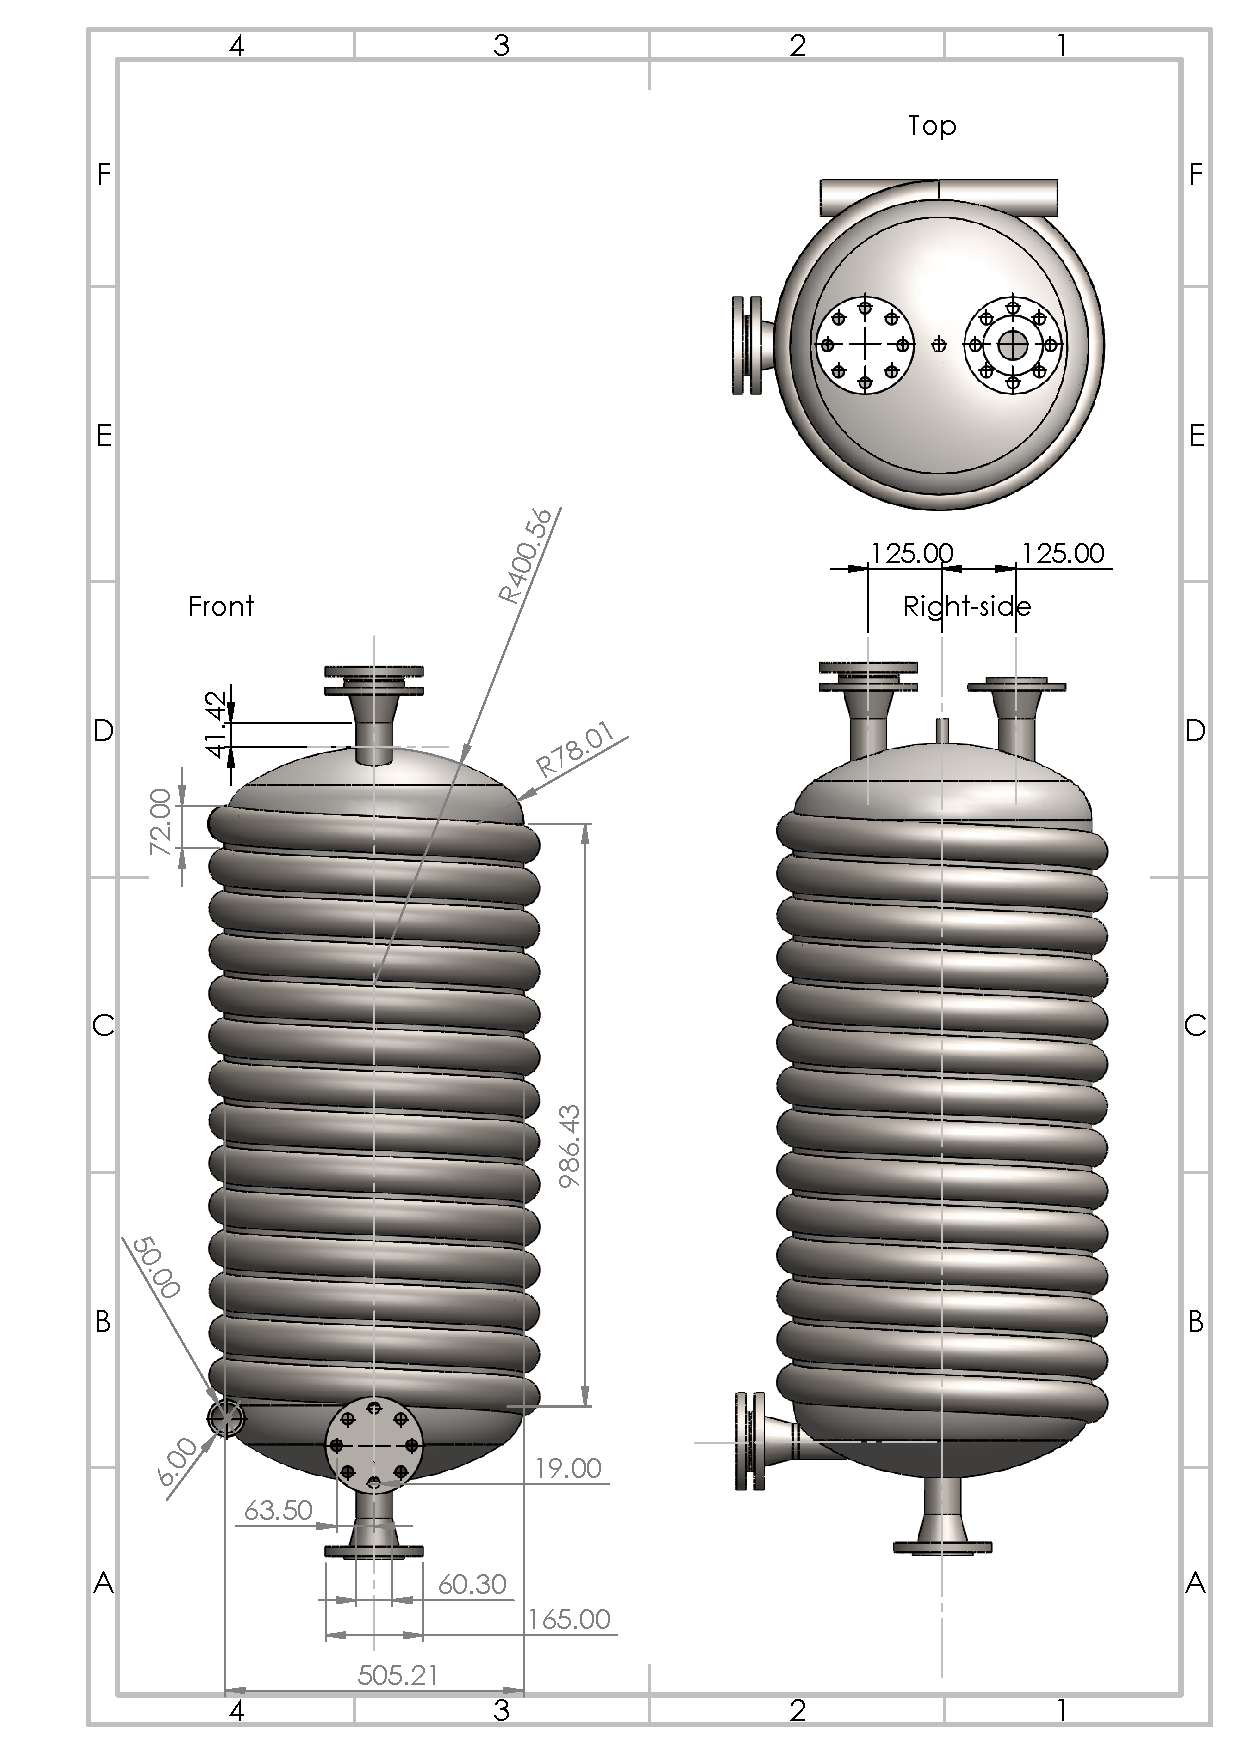
\includegraphics[scale=0.8]{chapters/3-separation/figures/Crystalliser_GA.PDF}
    \caption{GA drawing for the crystalliser vessel}
    \label{fig:crystalliser GA}
\end{figure} 

\newpage
\subsection{Conclusions and recommendations} \label{crystalliser conclusions}
